% day2_seg2_ranproc2/markov_proc.tex
\begin{frame}
  \onslide<1->{
	\frametitle{Some Important Random Processes} 
	\framesubtitle{Second Order Processes}
}
\begin{itemize}
  \onslide<2->{
 \item We will generally restrict our attention to \textit{\textbf{second-order processes}}, i.e., those such that
 $X(t)\in L^2(\Omega)$.
 \item Recall what this means:
 \[\expect{X^2(t)}<\infty\]
}
  \onslide<3->{
 \item This allows us to use Hilbert space techniques because, for
 every $s,t\in[0,T]$, $\expect{X(s)Y(t)}$ is an inner
 product.  Inner products, norms and metrics allow us to do
 calculus and geometry (orthogonal projection).
}
\end{itemize}
\end{frame}

\begin{frame}
  \onslide<1->{
	\frametitle{Some Important Random Processes} 
	\framesubtitle{Orthogonal Projection}
}
\begin{center}
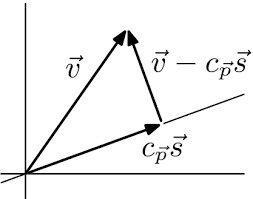
\includegraphics[scale=0.6]{graphics/orthoproj.png}
\end{center}
\end{frame}


\begin{frame}
  \onslide<1->{
	\frametitle{Some Important Random Processes} 
	\framesubtitle{Gaussian Processes}
}
\begin{itemize}
  \onslide<2->{
 \item An important class of second-order processes are the
 Gaussian processes.
}
  \onslide<3->{
\item Let $X:[0,T]\rightarrow L^2(\Omega)$ be a second-order
 process.  $X$ is said to be \textit{\textbf{Gaussian}} if for every finite set of times $\set{t_1,\ldots,t_n}$
 the vector of random variables $(X(t_1),\ldots,X(t_n))$ has a
 multivariate normal distribution.
}
  \onslide<4->{
  \item To fully appreciate what this means, we need to explain
 what a multivariate normal distribution is.
}
\end{itemize}
\end{frame}

\begin{frame}
  \onslide<1->{
	\frametitle{Some Important Random Processes} 
	\framesubtitle{Gaussian Processes}
}
\begin{itemize}
  \onslide<2->{
 \item A function $Q_C:\Real^n\rightarrow \Real$ of the form
 \[Q_C(x)=x\trans C x\]
 where $x\in\Real^n$ is a column vector and $C$ is a real symmetric
 matrix., is called a \textit{\textbf{quadratic form}} associated with $C$. (I.e., $C=(c_{ij})$ and $c_{ij}=c_{ji}$).
}
  \onslide<3->{
 \item We will further assume that $C$ is positive definite, which
 means that $Q_{C}(x)>0$ for every non-zero vector $x$.
}
\end{itemize}
\end{frame}

\begin{frame}
  \onslide<1->{
	\frametitle{Some Important Random Processes} 
	\framesubtitle{Gaussian Processes}
}
\begin{itemize}
  \onslide<2->{
 \item Then $X_1,\ldots,X_n$ are said to have a \textit{\textbf{multivariate normal distribution}}
 if their joint p.d.f. is of the form
\begin{equation}\label{gaussvec}
  f(x_1,\ldots,x_n)=\gvpdf
\end{equation}
for a real, positive definite symmetric matrix $C$ and
$\mu=(\mu_1,\ldots,\mu_n)$.
}
  \onslide<3->{
 \item $C$ is called the \textit{\textbf{covariance matrix}} and $\mu$ is called the
 \textit{\textbf{mean}} vector.
}
\end{itemize}
\end{frame}

\begin{frame}
  \onslide<1->{
	\frametitle{Some Important Random Processes} 
	\framesubtitle{Gaussian Processes}
}
\begin{itemize}
  \onslide<2->{
 \item In terms of quadratic forms, this is
 \[f(x_1,\ldots,x_n)= \sqrt{\frac{\det(C^{-1})}{(2\pi)^n }}
  \exp\left[ -\frac{1}{2}Q_{C^{-1}}(x-\mu) \right]\]
}
  \onslide<3->{
\item $C^{-1}$ is sometimes called the information matrix,
 because its inverse, the covariance matrix, often expresses the
 uncertainty (or lack of information) associated with the random
 variables.
}
\end{itemize}
\end{frame}

\begin{frame}
  \onslide<1->{
	\frametitle{Some Important Random Processes} 
	\framesubtitle{Gaussian Processes}
}
\begin{itemize}
  \onslide<2->{
\item Thus a Gaussian process is a random process for which the
 joint distribution of every finite collection of range random
 variables is a Gaussian distribution.
}
  \onslide<3->{
  \item The Gaussian process is important in connection with the
 kinds of noise that drive the dynamic systems we are interested
 in.
}
  \onslide<4->{
 \item The linear Kalman filter is optimal only under assumptions
 that the process noise and the measurement noise are Gaussian.
}
\end{itemize}
\end{frame}

\begin{frame}
  \onslide<1->{
	\frametitle{Some Important Random Processes} 
	\framesubtitle{Gauss-Markov Processes}
}
\begin{itemize}
  \onslide<2->{
 \item A Gauss-Markov process is for which the autocorrelation
 function has an exponential form:
\begin{equation}\label{gauss-markov}
  R_{XX}(\tau) = \sigma^2\exp(-\beta\abs{\tau})
\end{equation}
}
  \onslide<3->{
\item As a continuous-time dynamic system, this would correspond to passing white
 noise through first-order feedback system:
 \[\dot{x}=-\beta x+w\]
 \item See Matlab Simulink file gauss\_markov.mdl
}
\end{itemize}
\end{frame}

\begin{frame}
  \onslide<1->{
	\frametitle{Some Important Random Processes} 
	\framesubtitle{Gauss-Markov Processes}
}
\begin{itemize}
  \onslide<2->{
\item Discrete version of a Gauss-Markov process:
\[
x(k+1)=\exp\left(-\beta \Delta t\right)x(k) + w(k)
\]
where $\Delta t = t_{k+1}-t_k$ and is assumed to be the same regardless of $k$, and $w(k)$ is a white noise sequence
}
\end{itemize}
\end{frame}
\begin{frame}
  \onslide<1->{
	\frametitle{Some Important Random Processes} 
	\framesubtitle{Gauss-Markov Processes:  Simulink Model}
}
\begin{center}
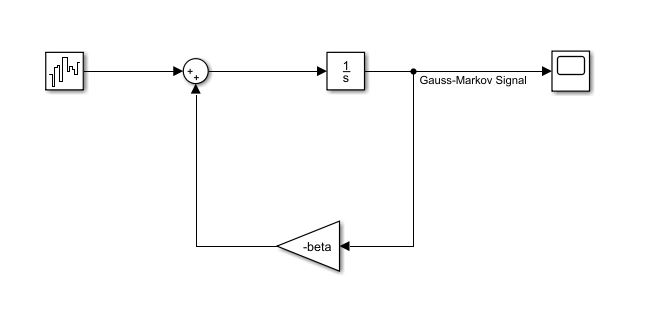
\includegraphics[scale=0.60]{day2_seg2_ranproc2/gauss_markov.jpg}
\end{center}
\end{frame}
\begin{frame}
  \onslide<1->{
	\frametitle{Some Important Random Processes} 
	\framesubtitle{Gauss-Markov Processes:  Output of Simulink Model}
}
\begin{center}
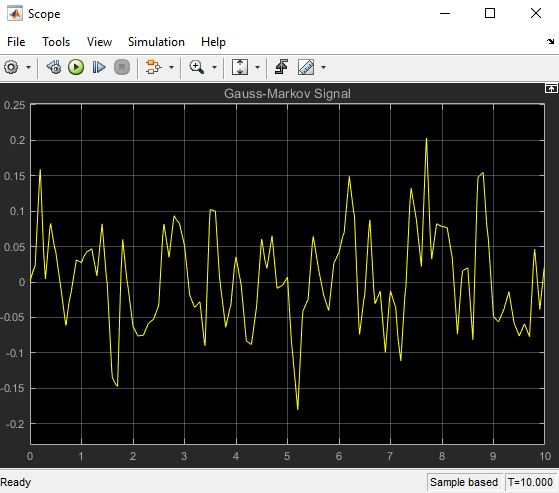
\includegraphics[scale=0.50]{day2_seg2_ranproc2/gauss_markov_scope.jpg}
\end{center}
\end{frame}
